%!TEX root = ../TTK4550-MHT.tex
\section{Linear programming}
\label{sec:ilp}
The aim of this section is to elaborate the use of linear programming to solve the data association problem in MHT that arises when there are multiple (possible mutual exclusive) possibilities of measurement arrangements within the existing set of tracks. As with any optimization problem, we need an objective function which tells us how good or bad a given assignment is, and a set of constraints that limits the solution to physical limits and our assumptions.

\subsection{Problem formulation}
Multiple optimization formulations of the association problem for multi target tracking have been proposed through the history. The first was \cite{Morefield1977} where a 0-1 ILP was proposed, followed by \cite{Storms2003} where an ILP scheme with LP relaxation and Greedy Rounding Procedure (GRP) as solvers were proposed and \cite{Coraluppi2004} were a framework for both association and removal of competing tracks.

All three mentioned publications have essentially equal objective functions, though some use minimize and other use maximize in their formulation. The essence of them all is (\ref{eq:general_objective_funtion}), where $\V{c}$ is a vector of costs (minimize) or scores (maximize) and $\V{x}$ (or $\V{\tau}$ as it is also commonly called) is a selection vector, where each row in $\V{c}$ and $\V{x}$ represents one branch in the track hypothesis tree.
\begin{equation}
\begin{aligned}
& \underset{x}{\text{min}}
& & \V{c}^T \V{x}
\end{aligned}
\label{eq:general_objective_funtion}
\end{equation}

Further, the constraints that shall ensure that each measurement is not assigned to more  than one track are generally formulated as (\ref{eq:general_constraints_equality}) or (\ref{eq:general_constraints_inequality}) , where $\M{A}$ is a binary matrix whose rows are branches in a track hypothesis tree and $\V{b}$ is a vector with ones.
\begin{equation}
\begin{aligned}
&	\M{A} \V{x} = \V{b} 	\\
&	\V{x} \in \{0,1\}
\end{aligned}
\label{eq:general_constraints_equality}
\end{equation}

\begin{equation}
\begin{aligned}
&	\M{A} \V{x} \leq \V{b} 	\\
&	\V{x} \in \{0,1\}
\end{aligned}
\label{eq:general_constraints_inequality}
\end{equation}
The difference between (\ref{eq:general_constraints_equality} and (\ref{eq:general_constraints_inequality}) originates from the   
\begin{equation}
\begin{aligned}
&	\underset{}{\text{maximize}}
&&	\V{c}^T \V{x} \\
&	\text{s.t.}
&&	\M{A_1} \V{x} \leq \V{b_1} 	\\
&&&	\M{A_2} \V{x} = \V{b_2}	\\
&&&	\V{x} \in \{0,1\}
\end{aligned}
\end{equation}
Where $\M{A_1}$ is a $N_1 \times M$ binary matrix with $N_1$ real measurements and $M$ track hypotheses (all leaf nodes), where $\M{A_1}(i,j)=1$ if hypothesis $j$ are utilizing measurement $i$, $0$ otherwise. The measurements and hypothesis are indexed by the order they are visited by a depth first search (DFS). $\M{A_2}$ is a $N_2 \times M$ binary matrix where $N_2$ is the number of targets in the cluster and $\M{A_2}(i,j)=1$ if hypothesis $j$ belongs to target $i$. $\V{b_1}$ is a $N_1$ long vector with ones and $\V{b_2}$ is a $N_2$ long vector with ones. $\V{c}$ is a $N$ long vector with a measure of the goodness of the track hypotheses. For example in Figure \ref{fig:hyp-tree} at time step 2, the A matrices  and C vector would be:
\begin{equation}
\begin{split}
\M{A_1} &=\begin{bmatrix}
		0 & 1 & 1 & 0 & 0 & 0 & 0 & 0 & 0 \\
       	0 & 0 & 1 & 0 & 0 & 1 & 0 & 1 & 0 \\
       	0 & 0 & 0 & 1 & 0 & 0 & 1 & 1 & 1 \\
       	0 & 0 & 0 & 0 & 0 & 0 & 0 & 0 & 1 \\
     	\end{bmatrix}
\V{b_1} = 	\begin{bmatrix}
			1 \\ 1  \\ 1 \\ 1
			\end{bmatrix} \\
\M{A_2} &=\begin{bmatrix}
		1 & 1 & 1 & 1 & 0 & 0 & 0 & 0 & 0 \\
       	0 & 0 & 0 & 0 & 1 & 1 & 1 & 1 & 1 \\
     	\end{bmatrix} 
\V{b_2} = 	\begin{bmatrix}
			1 \\ 1
			\end{bmatrix} \\
\V{c} &=\begin{bmatrix}
		\lambda_1 & \lambda_2 & \lambda_3 & \lambda_4 & \lambda_5 & \lambda_6 & \lambda_7 & \lambda_8 & \lambda_9
		\end{bmatrix}^T \\
\end{split}
\end{equation}

\begin{figure}
\centering
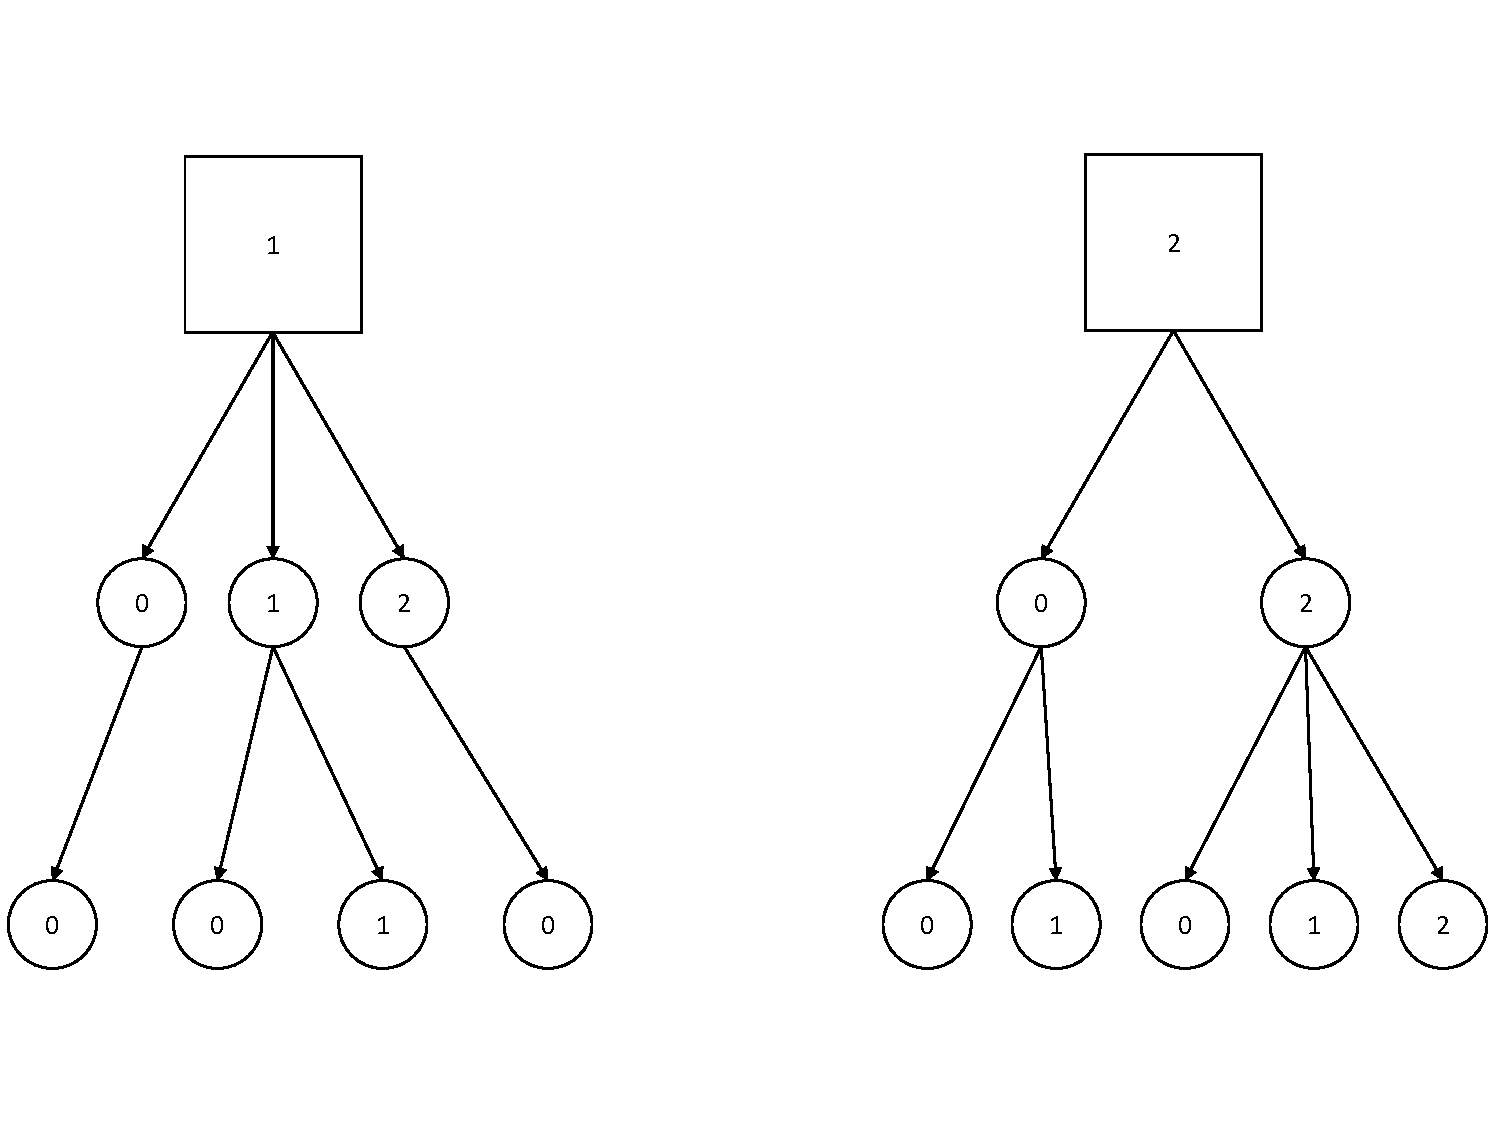
\includegraphics[width = .8\textwidth]{Track-tree}
\caption{Track hypothesis tree}
\label{fig:hyp-tree}
\end{figure}

\subsection{Solvers}
There are a lot of of-the-shelf integer linear program (ILP) and mixed integer linear program (MILP) solvers on the marked, both free open source and commercial. Since our problem is formulated on standard form, it can easily be executed on several solvers, and we can compare runtime and performance. In this report, the following solver are tested:
\begin{itemize}
\item CBC 		(Free, COIN-OR)
\item CPLEX 	(Commercial (Free academic),  IBM)
\item GLPK 		(Free, GNU)
\item Gurobi 	(Commercial (Free academic), Gurobi)
\end{itemize}

















